\documentclass[a4paper,5pt]{amsbook}
%%%%%%%%%%%%%%%%%%%%%%%%%%%%%%%%%%%%%%%%%%%%%%%%%%%%%%%%%%%%%%%%%%%%%

\usepackage{booktabs}
\usepackage{graphicx}
\usepackage{multicol}
\usepackage{textcomp}
\usepackage{systeme}
\usepackage{amssymb}
\usepackage[]{amsmath}
\usepackage{subcaption}
\usepackage[inline]{enumitem}
\usepackage{gensymb}

%%%%%%%%%%%%%%%%%%%%%%%%%%%%%%%%%%%%%%%%%%%%%%%%%%%%%%%%%%%%%%

\newcommand{\sen}{\,\mbox{sen}}
\newcommand{\tg}{\,\mbox{tg}\,}
\newcommand{\cosec}{\,\mbox{cosec}\,}
\newcommand{\cotg}{\,\mbox{cotg}\,}
\newcommand{\tr}{\,\mbox{tr}\,}
\newcommand{\ds}{\displaystyle}
\newcommand{\ra}{\rightarrow}

%%%%%%%%%%%%%%%%%%%%%%%%%%%%%%%%%%%%%%%%%%%%%%%%%%%%%%%%%%%%%%%%%%%%%%%%

\setlength{\textwidth}{16cm} %\setlength{\topmargin}{-1.3cm}
\setlength{\textheight}{25cm}
\setlength{\leftmargin}{1.2cm} \setlength{\rightmargin}{1.2cm}
\setlength{\oddsidemargin}{0cm}\setlength{\evensidemargin}{0cm}

%%%%%%%%%%%%%%%%%%%%%%%%%%%%%%%%%%%%%%%%%%%%%%%%%%%%%%%%%%%%%%%%%%%%%%%%

% \renewcommand{\baselinestretch}{1.6}
% \renewcommand{\thefootnote}{\fnsymbol{footnote}}
% \renewcommand{\theequation}{\thesection.\arabic{equation}}
% \setlength{\voffset}{-50pt}
% \numberwithin{equation}{chapter}

%%%%%%%%%%%%%%%%%%%%%%%%%%%%%%%%%%%%%%%%%%%%%%%%%%%%%%%%%%%%%%%%%%%%%%%

\begin{document}
\thispagestyle{empty}
\pagestyle{empty}
\begin{minipage}[h]{0.14\textwidth}
	
\includegraphics[scale=0.24]{../../ufgd.png}
\end{minipage}
\begin{minipage}[h]{\textwidth}
\begin{tabular}{c}
{{\bf UNIVERSIDADE FEDERAL DA GRANDE DOURADOS}}\\
{{\bf C\'alculo Diferencial e Integral III --- Lista 12}}\\
{{\bf Prof.\ Adriano Barbosa}}\\
\end{tabular}
\vspace{-0.45cm}
%
\end{minipage}

%------------------------

\vspace{1cm}
%%%%%%%%%%%%%%%%%%%%%%%%%%%%%%%%   formulario  inicio  %%%%%%%%%%%%%%%%%%%%%%%%%%%%%%%%
\begin{enumerate}
    \setlength\itemsep{0.5cm}
    \item Calcule a integral de linha $\int_C F\cdot\ dr$.
        \begin{enumerate}
            \setlength\itemsep{0.3cm}
            \item $F(x,y,z) = (x+y, y-z, z^2)$, $r(t)=(t^2, t^3, t^2)$, $0\le
            t\le 1$
            \item $F(x,y,z) = (\sen{x}, \cos{y}, xz)$, $r(t)=(t^3,-t^2,t)$,
            $0\le t\le 1$
            \item $F(x,y,z) = (x, y, -xz)$, $r(t)=(\cos{t},\sen{t},t)$, $0\le
            t\le \pi$
         \end{enumerate}

    \item Calcule o trabalho realizado pelo campo $F(x,y,z) = (x-y^2, y-z^2,
    z-x^2)$ ao mover uma part\'{\i}cula ao longo do segmento de reta que liga os
    pontos $(0,0,1$ e $(2,1,0)$.

    \item Determine se $F$ \'e um campo conservativo e calcule sua fun\c{c}\~ao
    potencial quando poss\'{\i}vel.
        \begin{enumerate}
            \setlength\itemsep{0.3cm}
            \item $F(x,y) = (2x-3y, -3x+4y-8)$
            \item $F(x,y) = (e^x \cos{y}, e^x\sen{y})$
            \item $F(x,y) = (ye^x+\sen{y}, e^x+x\cos{y})$
            \item $F(x,y) = (\ln{y}+2xy^3, 3x^2y^2+x/y)$
        \end{enumerate}

    \item A figura abaixo mostra o campo $F(x,y) = (2xy,x^2)$ e tr\^es curvas que
    come\c{c}am em $(1,2)$ e terminam em $(3,2)$. Explique por que $\int_C F\cdot\
    dr$ tem o mesmo valor para as tr\^es curvas. Qual \'e esse valor?
    \begin{figure}[h]
        \centering
        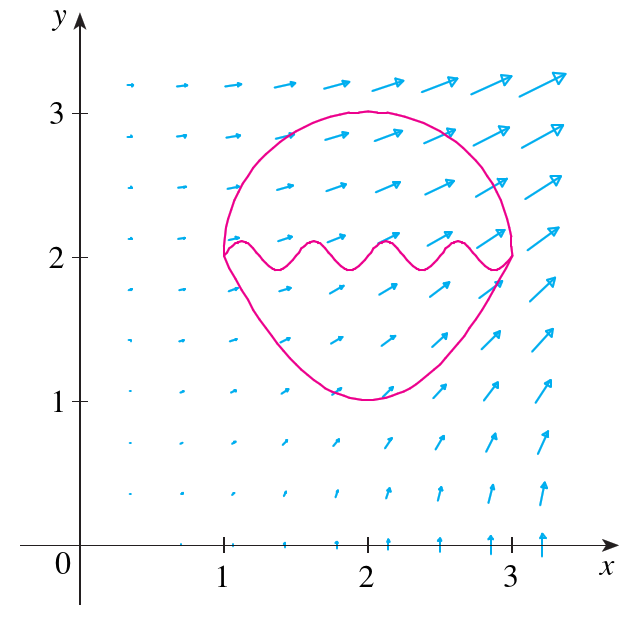
\includegraphics[width=0.4\textwidth]{lista-12-fig1.png}
    \end{figure}

    \item Determine o valor da integral $\int_C F\cdot\ dr$. Determine a fun\c{c}\~ao
    $f$ tal que $F=\nabla f$ antes de calcular a integral.
        \begin{enumerate}
            \setlength\itemsep{0.3cm}
            \item $F(x,y) = (x^2,y^2)$, onde $C$ \'e o arco da par\'abola $y=2x^2$
            de $(-1,2)$ e $(2,8)$
            \item $F(x,y) = (xy^2, x^2y)$, $C: r(t)=\left(t+\sen{\frac{1}{2}\pi
            t}, t+\cos{\frac{1}{2}\pi t}\right)$, $0\le t\le 1$
            \item $F(x,y,z) = (yz, xz, xy+2z)$, $C$ \'e o segmento de reta de
            $(1,0,-2)$ a $(4,5,3)$
        \end{enumerate}
\end{enumerate}

\end{document}
